\section{Auswertung}
\label{sec:Auswertung}
\subsection{Temperaturverläufe}
Die gemessenen Temperaturen $T_1$ und $T_2$ der Reservoire werden gegen die Zeit $t$ aufgetragen, um den Temperaturverlauf in den Reservoiren zu skizzieren.
Dabei ist Reservoir $R_1$ das Behältnis, welches die Wärmemenge $Q_1$ aufnimmt und sich dabei erhitzt; $R_2$ bezeichnet das kälter werdende Reservoir.  

\begin{table}
	\centering
	\sisetup{table-format=2.3}
	\begin{tabular}{S[table-format=1.2] S[table-format=1.3] S[table-format=1.3] }
	\toprule
	\multicolumn{1}{c}{Zeit} & {Temperaturen} \\
	{$t/\:\si{\minute}$} & {$T_1/\:\si{\kelvin}$} & {${T_2}/\:\si{\kelvin}$} \\
	\midrule
 0 & 294.45 & 294.45 \\
 1 & 295.35 & 294.45 \\
 2 & 296.15 & 294.35 \\
 3 & 297.45 & 293.45 \\
 4 & 299.05 & 292.05 \\
 5 & 300.85 & 290.25 \\
 6 & 302.95 & 288.25 \\
 7 & 304.85 & 286.45 \\
 8 & 306.85 & 284.65 \\
 9 & 308.65 & 282.85 \\
10 & 310.55 & 281.15 \\
11 & 312.25 & 279.45 \\
12 & 314.05 & 277.75 \\
13 & 315.65 & 276.35 \\
14 & 317.35 & 274.95 \\
15 & 318.85 & 273.95 \\
16 & 320.35 & 273.35 \\
17 & 321.75 & 272.85 \\
18 & 322.95 & 272.45 \\
19 & 324.15 & 272.05 \\
	\bottomrule
	\end{tabular}
	\caption{Zeitabhängige Messung der Temperaturen $T_1$ und $T_2$.}
	\label{tab:Temperaturverlauf}
\end{table}
\newpage
\noindent Werden die Verläufe in einem gemeinsamen Diagramm dargestellt, so lassen sich diese untereinander vergleichen. 

\begin{figure}
	\centering
	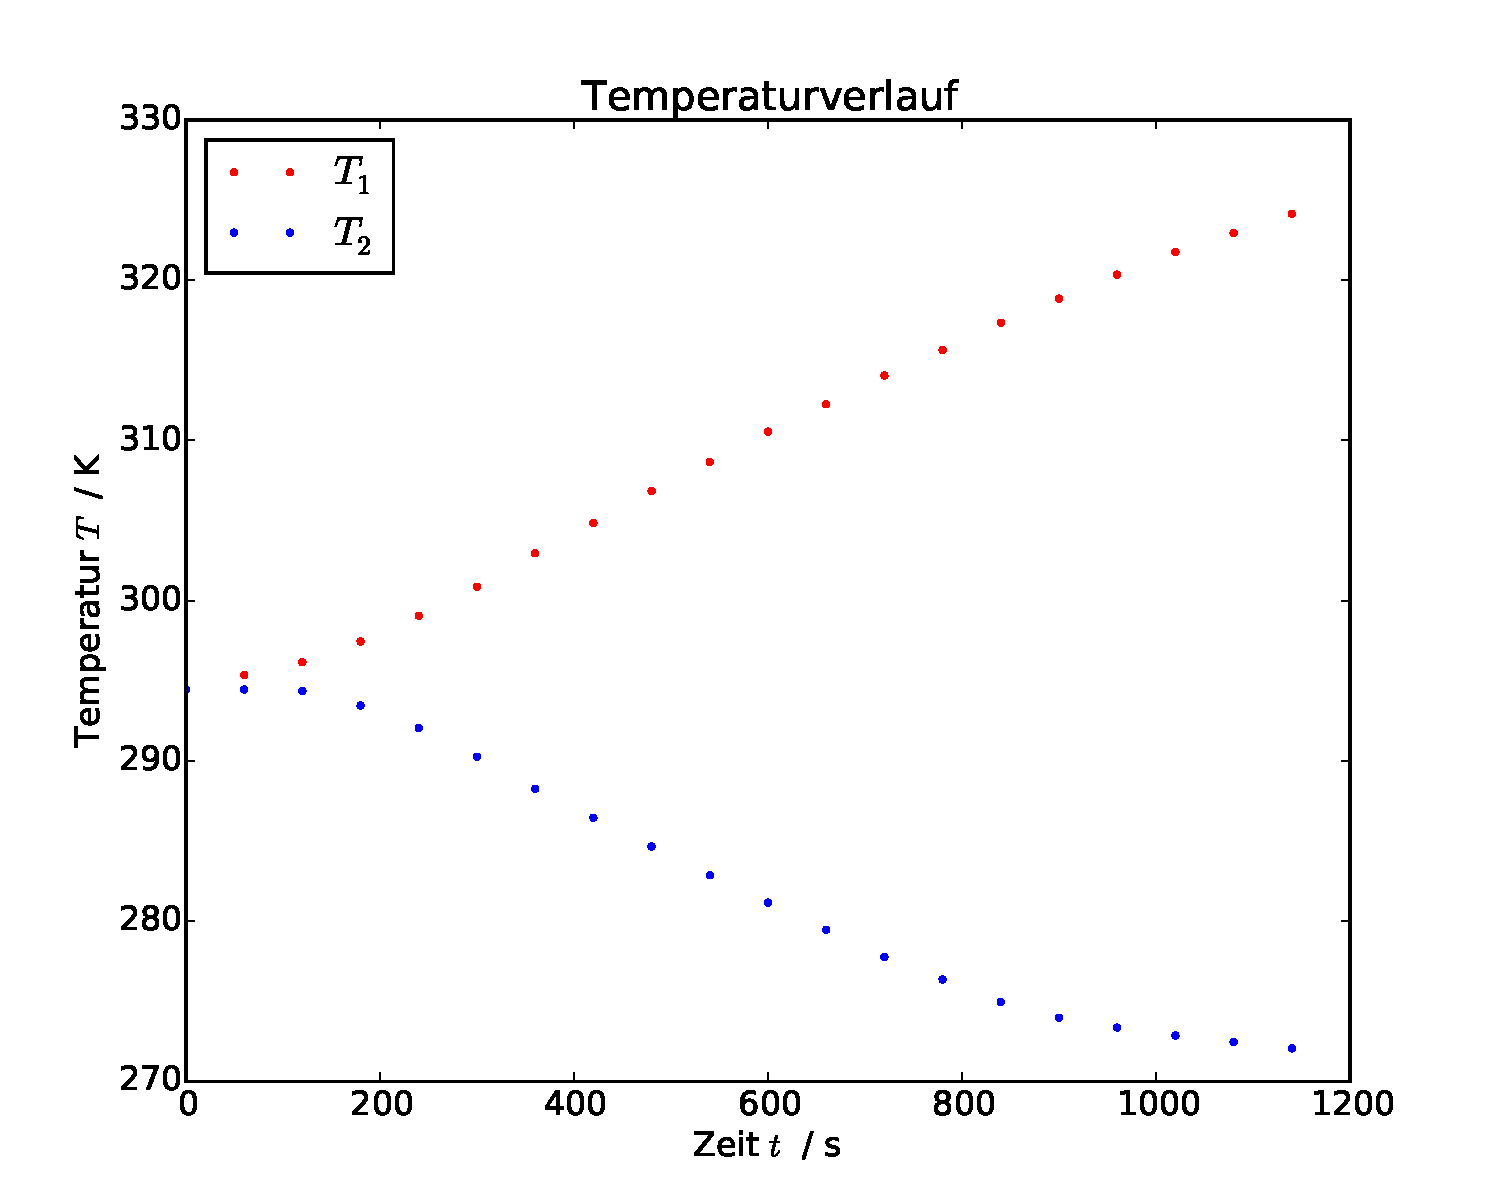
\includegraphics[width=0.9\textwidth]{Bilder/Temperaturverlauf.pdf}
	\caption{Entwicklung der Wassertemperatur in den Reservoiren $\mathup{R_1}$ und $\mathup{R_2}$.}
	\label{fig:temperaturverlauf}
\end{figure}

Der Temperaturverlauf wird nicht hinreichend gut durch die Funktionenklasse
\begin{equation}
	T_i(t)=A_i t² + B_i t + C_i , i=1,2
	\label{eq:t-verlauf_Grad2}
\end{equation}
genähert. 
\begin{figure}
	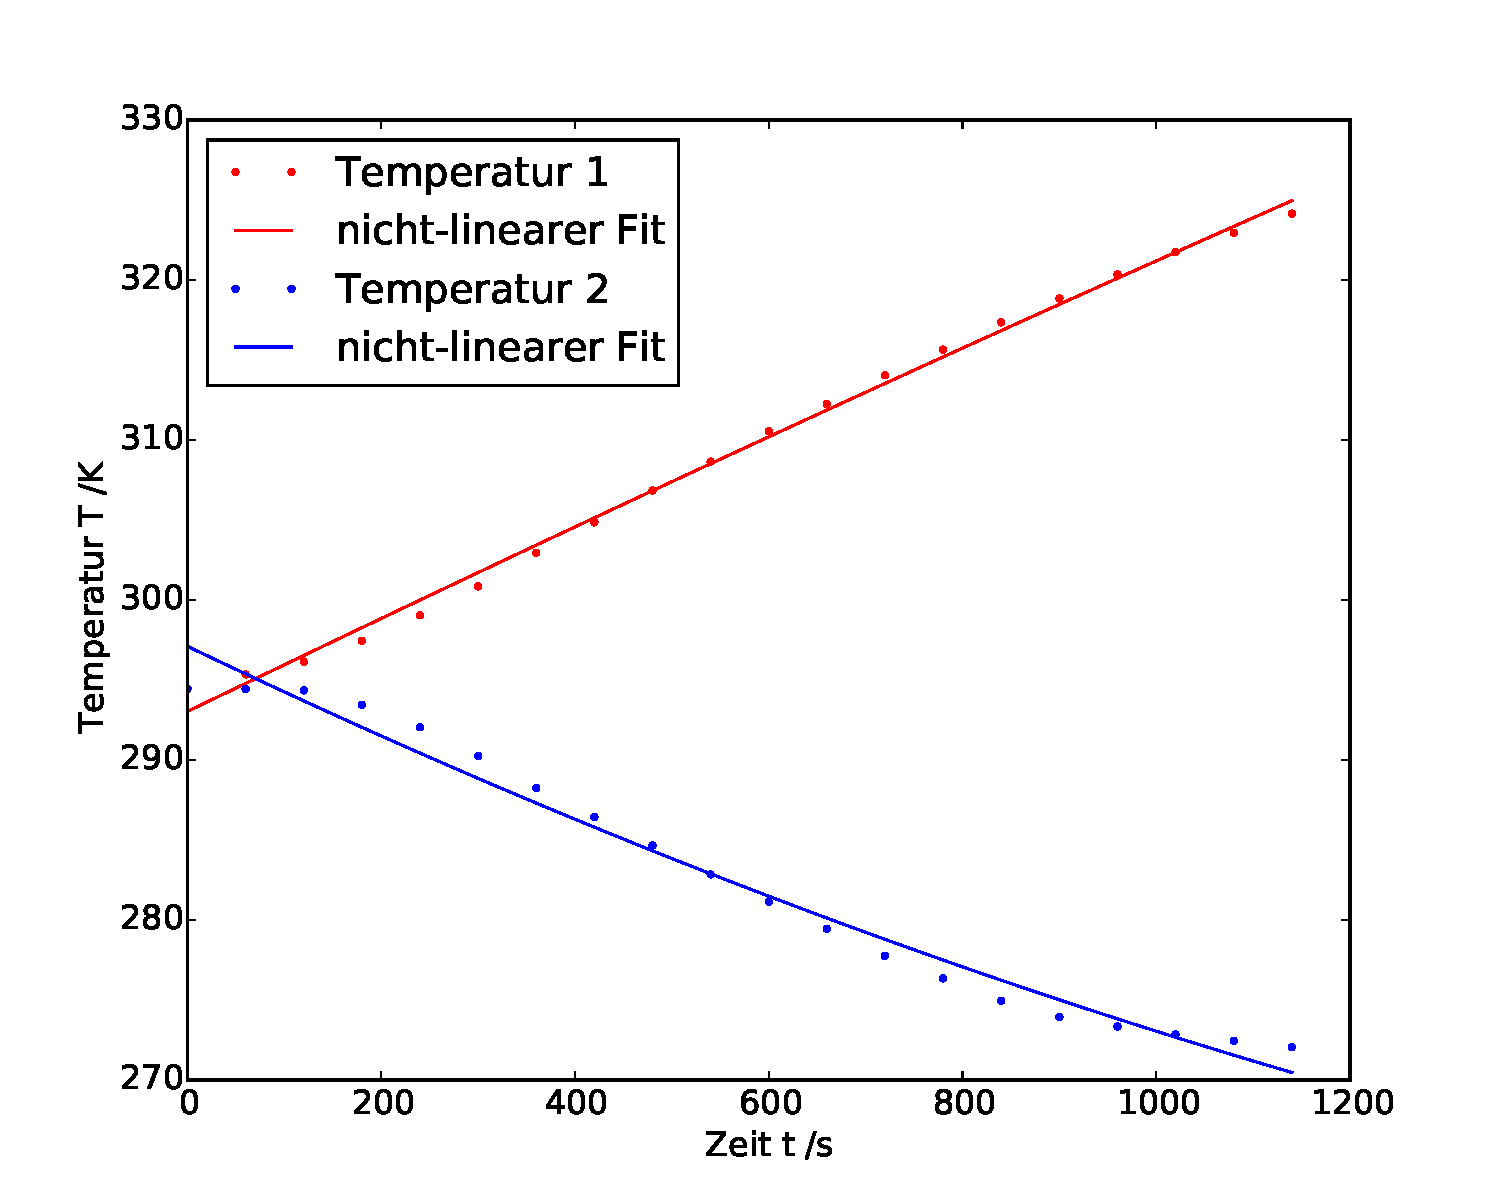
\includegraphics[width=\textwidth]{Bilder/Temperaturfit_Grad2.pdf}
	\caption{Annäherung der Kurven durch ein Polynom zweiter Ordnung.}
\end{figure}
\newpage
Trotz zweiter Ordnung erscheint die Ausgleichskurve annähernd linear.
Da schon anhand der Messwerte zu erkennen ist, dass diese einen Wendepunkt aufweisen, wird ein Polynom dritten Grades benutzt. 
\begin{equation}
	T_i(t)=A_i t³ + B_i t² + C_i t + D_i , i=1,2
	\label{eq:t-verlauf_Grad3}
\end{equation}
Die Näherung beschreibt die Messwerte wesentlich besser (vgl. Abbildung 2, 3). 

Es ergeben sich für $T_1(t)$ und $T_2(t)$ die Koeffizienten 
\begin{align}
	A_1&=(-1.72\pm0.18)10⁻⁸\,\si{\kelvin\per{\second}³}  & A_2&=(3.39\pm0.25)10⁻⁸\,\si{\kelvin\per{\second}³}\\
	B_1&=(2.82\pm0.31)10⁻⁵\,\si{\kelvin\per{\second}²}  & B_2&=(-5.30\pm0.43)10⁻⁵\,\si{\kelvin\per{\second}²}\\
	C_1&=(0.0162\pm0.0015)\,\si{\kelvin\per{\second}}  & C_2&=(-0.0033\pm0.0021)\,\si{\kelvin\per{\second}}\\
	D_1&=(294.11\pm0.19)\,\si{\kelvin}  & D_2&=(294.98\pm0.27)\,\si{\kelvin}.
\end{align}

Um den Differentialquotionenten $\frac{\mathup{d}T_i}{\mathup{d}t}$ mit $i=1,2$ für verschiedene Zeiten $t_k$ mit \\
$k= 1,...,4$ bestimmen zu können, wird die Funktion $T_i(t)$ nach der Zeit $t$ abgeleitet und die Fehler der Gradienten mittels Gaußscher Fehlerfortpflanzung berechnet.
\begin{equation}
	\frac{\mathup{d}T_i}{\mathup{d}t}= 3A_it²+2B_it+C_i.
	\label{ableitung}
\end{equation}
\begin{figure}
	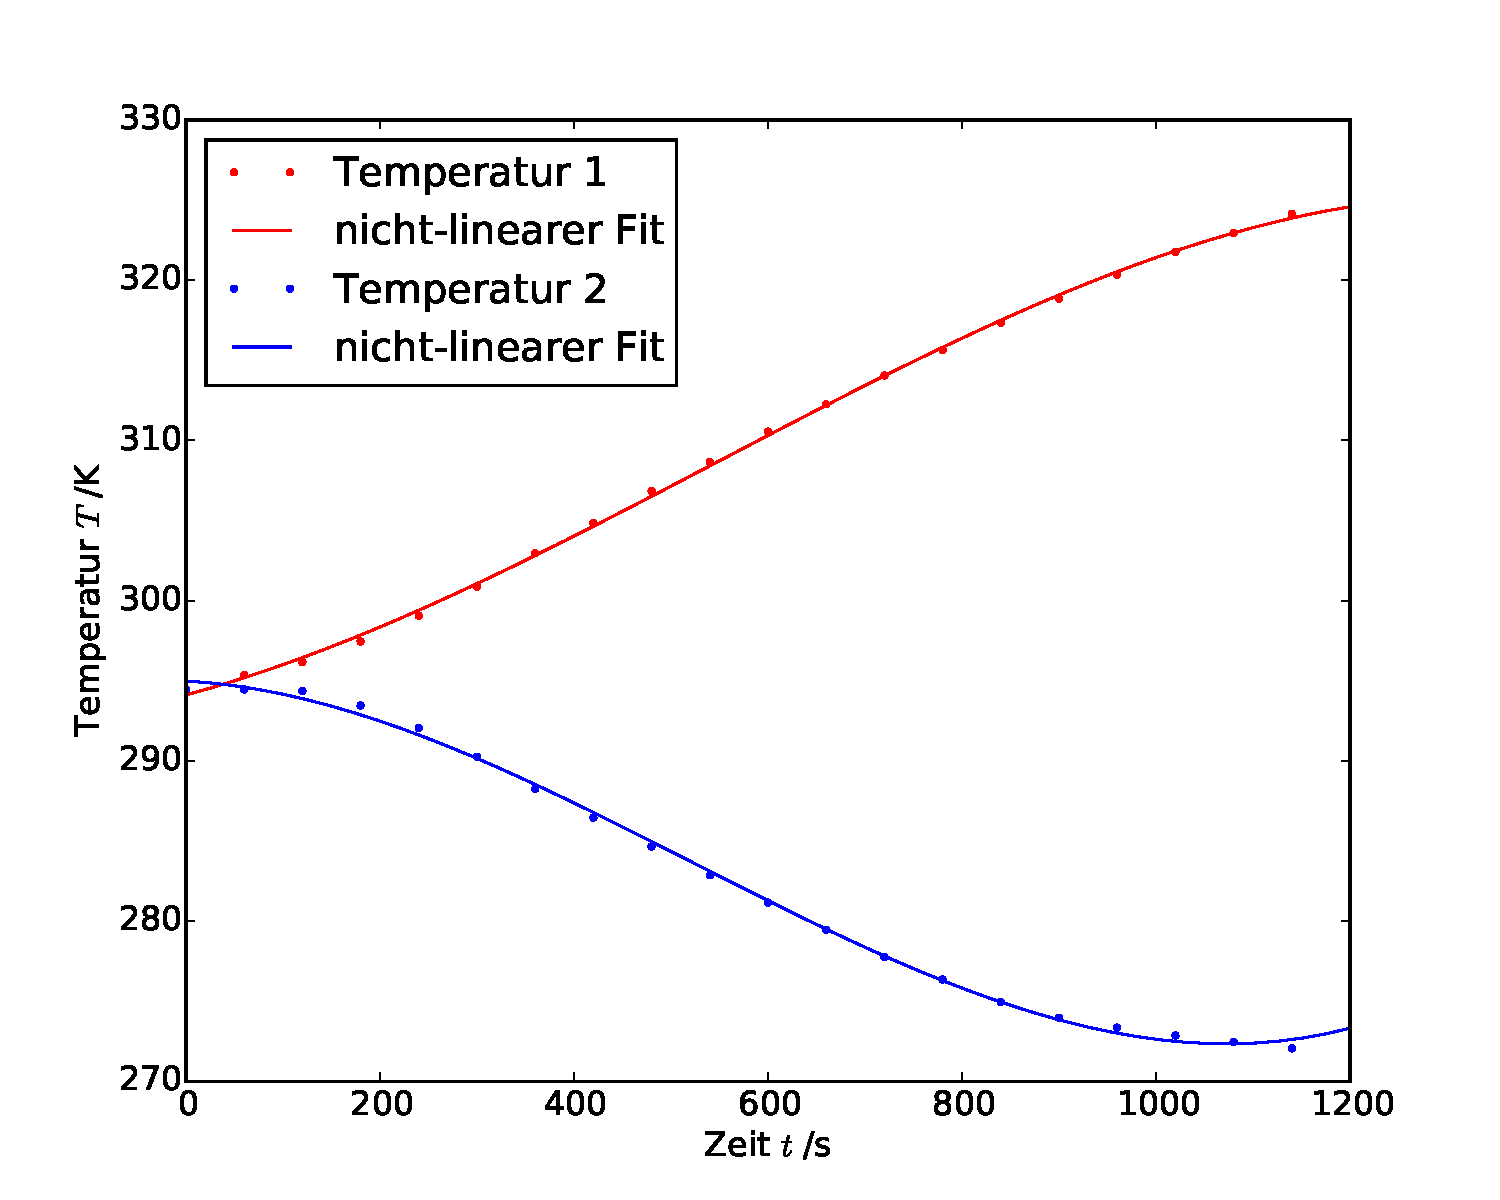
\includegraphics[width=\textwidth]{Bilder/Temperaturfit.pdf}
	\caption{Annäherung der Kurven durch ein Polynom dritter Ordnung.}
\end{figure}

\begin{table}
	\centering
	\begin{tabular}{S S S}
	\toprule
	\multicolumn{1}{c}{Zeit} & \multicolumn{2}{c}{Differentialquotienten} \\
	{$t/\:\si{\second}$} & {$\frac{\mathup{d}T_1}{\mathup{d}t}/\:\si{\kelvin{\per\second}}$} & {$\frac{\mathup{d}T_2}{\mathup{d}t}/\:\si{\kelvin{\per\second}}$}\\
	\midrule
 120 & 0.022 \pm 0.002   & -0.015 \pm 0.002  \\
 480 & 0.032 \pm 0.004   & -0.031 \pm 0.005  \\
 840 & 0.027 \pm 0.007   & -0.021 \pm 0.009  \\
 960 & 0.023 \pm 0.008   & -0.011 \pm 0.011  \\
	\bottomrule
	\end{tabular}
	\caption{Die Differentialqutienten von $T_1$ und $T_2$ zu vier verschiedenen Zeiten $t_k$, berechnet nach Gleichung \eqref{ableitung}.}
	\label{tab:differentialquotienten}
\end{table}


\newpage
\subsection{Bestimmung der Güteziffer}
Die reale Güteziffer $\nu$ wird mit Hilfe der Messreihe $T_1$ über \eqref{waermemenge/zeitintervall} berechnet.
Die Konstanten $c_\mathup{w}=4.183\cdot 10⁻³\:\si{\joule\per{\kelvin\kilo\gram}}$\cite{waermekapazitaet} und $m_\mathup{k}c_\mathup{k}=660\:\si{\joule\per\kelvin}$ sind die Wärmekapazitäten des verwendeten Wassers und der kupfernen Spirale.
Die Gesamtkapazität bei 3\,l Wasservolumen ist $m_1c_\mathup{w}+m_\mathup{k}c_\mathup{k}=13209\:\si{\joule\per\kelvin}$.

Die Fehlerangaben der werden berechnet mit
\begin{equation}
	\sigma_\nu=\Delta{\nu_\mathup{real}}=\sqrt{\biggl(\frac{(m_1c_\mathup{w}+m_\mathup{k}c_\mathup{k})\Delta\frac{\mathup{d}T_1}{\mathup{d}{t}}}{N_t}\biggr)^2+\biggl(\frac{(m_1c_\mathup{w}+m_\mathup{k}c_\mathup{k})\Delta{T_1}}{N_t^2 \Delta{t}}\Delta{N_t}\biggr)^2},
\end{equation}
wobei $\Delta{N_t}$ der mittlere Fehler von $N_t$ ist (vgl. \ref{tab:differentialquotienten}). 
Beides wird berechnet durch
\begin{equation}
	N_t=\frac{1}{n}\sum_{k=0}^n{(N_k-N)²},
\end{equation}
\begin{equation}
	\Delta{N_t}=\sqrt{\frac{\frac{1}{n-1}\sum_{k=0}^n(N_k)}{n}}.
\end{equation}

Die ideale Güteziffer $\nu_\mathup{ideal}$ wird zum Vergleich nach Gleichung \eqref{eq:gueteziffer_ideal} zum Vergleich berechnet.

\begin{table}
	\centering
	\begin{tabular}{S S S}
	\toprule
	{Zeit} & \multicolumn{2}{c}{Güteziffern} \\
	{$t/\:\si{\second}$} & {$\nu_\mathup{real}$} & {$\nu_\mathup{ideal}$} \\
	\midrule
 120 & 0.873 \pm 0.081   & 164.528  \\
 480 & 1.252 \pm 0.159   &  13.822 \\
 840 & 1.057 \pm 0.275   &   7.485 \\
 960 & 0.900 \pm 0.314   &   6.816 \\
	\bottomrule
	\end{tabular}
	\caption{Die realen und idealen Güteziffern zu vier verschiedenen Zeiten $t_k$ im Vergleich.}
	\label{tab:gueteziffern}
\end{table}
\newpage
\subsection{Bestimmung des Massendurchsatzes}

\begin{table}
	\centering
	\begin{tabular}{S S S}
	\toprule
	\multicolumn {1}{c}{Zeit} & \multicolumn {2}{c}{Druck} \\
	{$t/\:\si{\minute}$} & {$p_\mathup{a}/\:\si{\bar}$} & {$p_\mathup{b}/\:\si{\bar}$} \\
	\midrule
00 &1.00 & 01.00\\
01 &2.40 & 07.00\\
02 &2.60 & 07.00\\
03 &2.85 & 07.50\\
03 &3.00 & 07.75\\
05 &3.20 & 08.00\\
06 &3.20 & 08.50\\
07 &3.20 & 09.00\\
08 &3.20 & 09.50\\
09 &3.20 & 09.75\\
10 &3.20 & 10.00\\
11 &3.20 & 10.50\\
12 &3.20 & 11.00\\
13 &3.20 & 11.25\\
14 &3.20 & 11.50\\
15 &3.20 & 12.00\\
16 &3.20 & 12.50\\
17 &3.20 & 12.75\\
18 &3.20 & 13.00\\
19 &3.20 & 13.25\\
	\bottomrule
	\end{tabular}
	\caption{Gemessene Drücke $\tilde{p}_\mathup{a}$, $\tilde{p}_\mathup{b}$, zu denen $1\si\bar$ Außendruck addiert wurde.}
	\label{tab:massendurchsaetze}
\end{table}

Dem Reservoir wird durch das verdampfende Gas die Wärmemenge $Q_2$ entzogen. 
Dabei wird die Verdampfungswärme $L$ verbraucht, welches über die Dampfdruckkurve des verwendeten Gases Dichlordifluormethan bestimmt wird. 
Wie in der Versuchsanleitung V203 beschrieben, wird der Druck $p_\mathup{b}$ gegen den Kehrwert der Temperatur $T_1$ aufgetragen.
Da die Manometer den Außendruck von $1\si{\bar}$ nicht berücksichtigen, muss dieser zuvor noch zu den Messwerten addiert werden, wie in Tabelle \ref{tab:massendurchsaetze} geschehen. 
Mit linearer Regression werden anschließend Steigung $\mu$ und y-Achsenabschnitt $b$ der Gerade bestimmt. 
\begin{equation}
	\ln{(p_\mathup{b})}=\mu \frac{1}{T}+b=-\frac{L}{R}\frac{1}{T}+b
\end{equation}
$R$ ist die allgemeine Gaskonstante.

Die Steigung ist $\mu=-(2.093\pm0.050)10³\,\si\kelvin$, der Achsenabschnitt $b=(9.080\pm0.163)$.
Damit L die Einheit $\si{\joule\per{\kilo\gram}}$ besitzt, wird durch die molare Masse $M=120.9\,\si{\gram\per\mol}$ des Gases dividiert. 
Der Fehler der allgemeinen Gaskonstante $\text{R}=(8.314\pm 9.1\cdot10⁻⁷)\,\si{\joule\per{\mol\kelvin}}$ wird dabei vernachlässigt, der Fehler von L entspricht also dem Fehler von $\mu$.
Daraus ergibt sich $L=\frac{\lvert \mu\rvert \text{R}}{M}=143.913\pm0.050 \cdot10³\,\si{\joule\per\gram}$.

\begin{figure}
	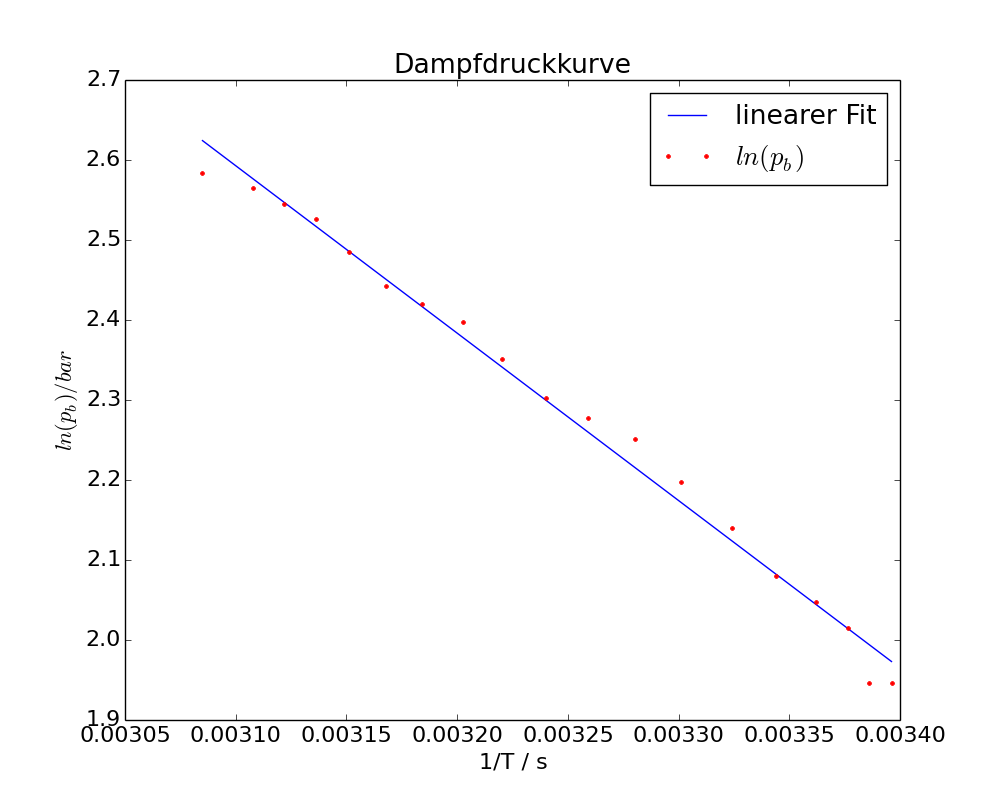
\includegraphics[width=\textwidth]{Bilder/Dampfdruckkurve.png}
	\caption{Dampfdruckkurve des Gases Dichlordiflourmethan.}
\end{figure}

Der Massendurchsatz $\frac{\Delta{m}}{\Delta{t}}$ wird berechnet mit den Gleichungen \eqref{eq:q2-t-verhaeltnis},\eqref{eq:verdampfungswaerme}.
Der Fehler wird ebenfalls nach Gauß berechnet mit dem Fehler der Verdampfungswärme $\Delta{L}$ und dem Fehler des Differentialquotienten $\Delta{\frac{\mathup{d}T_2}{\mathup{d}t}}$.
\begin{equation}
	\sigma_m=\sqrt{\biggl(\frac{(m_2c_\mathup{w}+m_\mathup{k}c_\mathup{k})\Delta\frac{\mathup{d}T_2}{\mathup{d}{t}}}{L}\biggr)^2+\biggl(\frac{(m_2c_\mathup{w}+m_\mathup{k}c_\mathup{k})\Delta{T_2}}{L^2 \Delta{t}}\Delta{L}\biggr)^2}
\end{equation}

\begin{table}
	\centering
	\begin{tabular}{S S}
	\toprule
	\multicolumn{1}{c}{Zeit} & \multicolumn{1}{c}{Massendurchsatz} \\
	{$t/\:\si{\second}$} & {$\frac{\Delta{m}}{\Delta{t}}/\:\si{\gram\per\second}$} \\
	\midrule
 120 & 1.4\pm 0.5\\
 480 & 3\pm 1\\
 840 & 2 \pm 1\\
1080 & 1\pm 1 \\
	\bottomrule
	\end{tabular}
	\caption{Massendurchsätze zu verschiedenen Zeiten.}
	\label{tab:massendurchsaetze}
\end{table}
\newpage
\subsection{Bestimmung der mechanischen Kompressorleistung}
Die mechanische Kompressorleistung wird mit Formel \eqref{eq:kompressorleistung} bestimmt.
Die Konstante $\kappa$ beträgt in diesem Fall $\kappa=1.14$. 
Die Dichte des Transportmediums kann über Gleichung \eqref{eq:transportmediumdichte} zu jeder beliebigen Temperatur $T_2$ berechnet werden.

\begin{table}
	\centering
	\begin{tabular}{S S c S S}
	\toprule
	{Zeit} & {Dichte} & \multicolumn{2}{c}{Kompressorleistungen} & {Wirkungsgrad}\\
	{$t/\:\si{\second}$} & {$\rho/\:\si{\kilo\gram\per{\cubic\meter}}$} & {$N_\mathup{m.}/\:\si\watt$} & {$N_\mathup{el.}/\:\si\watt$}& {\eta}\\
	\midrule
 120 & 13.294 & $25\pm  9.$ & 175 & 0.142\\
 480 & 16.920 & $55\pm 20$ & 205 & 0.268 \\
 840 & 17.517 & $43\pm 20$ & 210 & 0.204\\
 960 & 17.619 & $26\pm 30$ & 210 & 0.124\\
	\bottomrule
	\end{tabular}
	\caption{Elektrische und mechanische Kompressorleistung im Vergleich.}
	\label{tab:leistung}
\end{table}

Die Fehler werden analog wie zu den vorherigen Kapiteln nach Gauß berechnet.
\begin{equation}
\Delta{N_\mathup{m.}}=\frac{1}{\kappa-1}\biggl(p_\mathup{b}\sqrt[\kappa]{\frac{p_\mathup{a}}{p_\mathup{b}}}-p_\mathup{a}\biggr)\frac{1}{\rho} \sigma_m
\end{equation}
